\clearpage
\phantomsection
\vspace*{0.2cm}

مبانی نظری این معماری مبتنی بر دستاوردهای علمی \cite{ref_hymbatransx_2024} است.
\noindent\rule{\textwidth}{1.2pt}
\vspace*{0.1cm}
\section{تحلیل علمی و کالبدشکافی ساختاری ماژول \lr{hymba\_transx}}
\label{sec:mod_hymba_transx}
\vspace*{-0.2cm}
\noindent\rule{\textwidth}{0.5pt}
\vspace*{0.3cm}

\subsection*{بخش ۱: ایده محوری و چرایی معماری \lr{(Architectural Rationale)}}
توجه استاندارد ترنسفورمرها از پیچیدگی مجانبی $\mathcal{O}(N^2)$ نسبت به طول دنباله رنج می‌برد. ماژول \lr{HymbaTransX} به عنوان یک ساختار مرکب هیبریدی، ایده درهم‌آمیختن «توجه تفاضلی» \lr{(Differential Attention)} و «مدل فضای حالت» \lr{(State Space Model - SSM)} را مطرح می‌نماید. هدف اصلی این معماری، جبران نقاط ضعف مدل‌های مبتنی بر \lr{SSM} در بازیابی دقیق اطلاعات (استخراج انتخابی) با استفاده از یک مکانیزم توجه بسیار سبک‌وزن است. با فرمول‌بندی یک توجه تفاضلی از طریق تفریق دو نگاشت توجه \lr{Softmax} مجزا، مدل قادر به فیلترینگ مؤثرتر نویزها و افزایش نسبت سیگنال به نویز در ماتریس توجه می‌شود. همزمان، شاخه فضای حالت وظیفه ضبط و فشرده‌سازی زمینه سراسری توالی با پیچیدگی زمانی خطی $\mathcal{O}(N)$ را بر عهده می‌گیرد و ترکیب این دو، تعادلی بهینه میان دقت بازیابی اطلاعات و کارایی پردازشی برقرار می‌سازد.

\subsection*{بخش ۲: فرمول‌بندی ریاضی و مبانی نظری \lr{(Mathematical Formulation)}}
در این ساختار، تانسور ورودی $\mathbf{X} \in \mathbb{R}^{B \times N \times D}$ به طور موازی به هر دو شاخه توجه تفاضلی و فضای حالت خورانده می‌شود. 
برای شاخه توجه، دو مجموعه پرس‌وجو و کلید تولید می‌گردد:
\begin{align*}
\mathbf{Q}_1, \mathbf{K}_1 &= \text{\lr{RoPE}}(\mathbf{X}\mathbf{W}_{Q1}, \mathbf{X}\mathbf{W}_{K1}) \\
\mathbf{Q}_2, \mathbf{K}_2 &= \text{\lr{RoPE}}(\mathbf{X}\mathbf{W}_{Q2}, \mathbf{X}\mathbf{W}_{K2}) \\
\mathbf{V} &= \mathbf{X}\mathbf{W}_V
\end{align*}
در اینجا ماتریس‌های وزن پروجکشن با استفاده از آداپتورهای \lr{LoRA} فرمول‌بندی شده‌اند تا در طول آموزش‌های ثانویه از هزینه‌های محاسباتی کاسته شود. پس از نگاشت به ابعاد $[B, H, N, d]$ و اعمال کدگذاری مکانی چرخشی \lr{(RoPE)}، امتیازات توجه محاسبه می‌شود:
\begin{align*}
\mathbf{S}_1 &= \frac{\mathbf{Q}_1\mathbf{K}_1^\top}{\sqrt{d}}, \quad \mathbf{S}_2 = \frac{\mathbf{Q}_2\mathbf{K}_2^\top}{\sqrt{d}} \\
\mathbf{A}_{\text{\lr{diff}}} &= \text{\lr{ReLU}}\big(\text{\lr{Softmax}}(\mathbf{S}_1) - \lambda \cdot \text{\lr{Softmax}}(\mathbf{S}_2)\big)
\end{align*}
در این پیاده‌سازی، ضریب $\lambda = 0.2$ به عنوان ضریب تعدیل در نظر گرفته شده است. خروجی توجه به صورت $\mathbf{O}_{\text{\lr{attn}}} = \bar{\mathbf{A}}_{\text{\lr{diff}}} \mathbf{V}$ محاسبه می‌گردد (که در آن $\bar{\mathbf{A}}_{\text{\lr{diff}}}$ نمایانگر ماتریس پس از نرمال‌سازی مجموع در راستای سطرهاست).
در موازات، شاخه فضای حالت خروجی $\mathbf{O}_{\text{\lr{ssm}}} = \text{\lr{SSM}}(\mathbf{X})$ را تولید می‌کند و ترکیب نهایی به کمک یک پارامتر آموختنی $\alpha$ صورت می‌پذیرد:
\begin{equation}
\mathbf{O} = \big(\sigma(\alpha) \mathbf{O}_{\text{\lr{attn}}} + (1 - \sigma(\alpha)) \mathbf{O}_{\text{\lr{ssm}}}\big) \mathbf{W}_O
\end{equation}
پیچیدگی زمانی این رویکرد برابر $\mathcal{O}(N^2 d + N d)$ بوده و ترکیب خطی \lr{SSM} از بار سنگین حافظه برای زمینه‌های بسیار طولانی می‌کاهد.

\subsection*{بخش ۳: کالبدشکافی سورس‌کد و ردگیری تانسورها \lr{(Source Code \& Tensor Trace)}}
کلاس \lr{HymbaTransXBlock}، پیاده‌سازی رسمی این معماری است. ورودی $\mathbf{X}$ به ماژول‌های \lr{LoRALinear} با قابلیت فریز کردن پایه‌های وزنی ارسال می‌شود.
مراحل ردگیری تانسورها به شرح زیر است:
\begin{enumerate}
    \item \textbf{پروجکشن خطی و تغییر شکل:} تبدیل ورودی به پروجکشن‌های $\mathbf{Q}_1, \mathbf{K}_1, \mathbf{Q}_2, \mathbf{K}_2$ و $\mathbf{V}$ با ابعاد بازآرایی شده $[B, H, N, d]$.
    \item \textbf{اعمال \lr{RoPE}:} از طریق کلاس \lr{HeadRoPE}، رمزگذاری مکانی چرخشی به بردارهای $\mathbf{Q}$ و $\mathbf{K}$ اعمال می‌شود که در درک ارتباطات نسبی حیاتی است.
    \item \textbf{مکانیسم \lr{GQA}:} در صورت وجود سرهای پرس‌وجوی گروه‌بندی‌شده \lr{(GQA)}، تابع \lr{repeat\_kv} تانسورهای کلید و مقدار را برای تطبیق با ابعاد $\mathbf{Q}$ بسط می‌دهد.
    \item \textbf{توجه تفاضلی:} مقادیر \lr{Softmax} محاسبه شده و اختلاف آن‌ها گرفته می‌شود. با اعمال \lr{ReLU} و یک تجمیع مجموع روی بعد آخر \lr{(denom)}، مقادیر نرمال می‌شوند تا پایداری گرادیان در فاز پس‌انتشار حفظ شود.
    \item \textbf{ترکیب و خروجی:} تانسور خروجی توجه با خروجی \lr{SimpleSSM} به وسیله متغیر \lr{alpha} که از فیلتر سیگموید \lr{(Sigmoid)} گذشته است ترکیب خطی شده و نهایتاً از \lr{out\_proj} عبور می‌نماید.
\end{enumerate}

\subsection*{بخش ۴: تحلیل معماری سخت‌افزار و مدل سقف کارایی \lr{(Hardware \& Roofline Analysis)}}
از دیدگاه پردازنده گرافیکی \lr{NVIDIA GeForce RTX 4070 Laptop (8GB GDDR6)}، ماژول \lr{hymba\_transx} به دلیل اجرای موازی دو بلوک مجزا، شدت حسابی \lr{(Arithmetic Intensity)} بالاتری در مقایسه با \lr{SSM} خالص دارد. با این حال، استفاده از سرهای گروه‌بندی‌شده \lr{(GQA)} به میزان قابل توجهی ترافیک خوانش از حافظه با پهنای باند بالا \lr{(HBM)} را برای تانسورهای $\mathbf{K}$ و $\mathbf{V}$ کاهش می‌دهد و نرخ استفاده از حافظه \lr{SRAM} را برای کش‌سازی این تانسورها بهبود می‌بخشد.
از آنجا که عملیات توجه به دلیل مجذور طول توالی \lr{Memory-Bound} و عملیات \lr{SSM} به خاطر اسکن‌های بازگشتی ممکن است \lr{Compute-Bound} باشد، توزیع این دو بلوک به تعادل خط لوله محاسبات پردازنده کمک کرده و در طول دنباله‌های تا ۲۰۴۸ توکن، توان عملیاتی بالایی را بدون رخداد گلوگاه پهنای باند حافظه تضمین می‌نماید.

\subsection*{بخش ۵: کارنامه تجربی و ارزیابی آزمایشگاهی \lr{(Empirical Results \& Benchmark)}}
عملکرد ماژول \lr{hymba\_transx} بر پایه ارزیابی‌های جامع تجربی بر روی بنچ‌مارک \lr{GLUE} شامل دادگان \lr{SST-2} و \lr{MRPC} به شرح جدول زیر می‌باشد. مقادیر ثبت شده بازتاب مستقیمی از تعامل این مکانیزم با معماری‌های پایه‌ای مختلف است:

\begin{table}[H]
\centering
\small
\caption{عملکرد آزمایشگاهی ماژول \lr{hymba\_transx} بر روی مجموعه داده‌های \lr{SST-2} و \lr{MRPC}}
\label{tab:benchmark_hymba_transx}
\begin{tabular}{lccc}
\toprule
\textbf{مدل پایه} & \textbf{دقت \lr{SST-2}} & \textbf{دقت \lr{MRPC}} & \textbf{شاخص \lr{F1} \lr{(MRPC)}} \\
\midrule
\lr{DistilBERT} & \lr{89.79\%} & \lr{84.31\%} & \lr{89.20\%} \\
\lr{RoBERTa-base} & \lr{93.80\%} & \lr{86.51\%} & \lr{90.67\%} \\
\lr{GPT-2} & \lr{89.44\%} & \lr{81.61\%} & \lr{86.54\%} \\
\bottomrule
\end{tabular}
\end{table}

\subsection*{بخش ۶: تحلیل و تفسیر نتایج و رفتار رده‌های کلاسی \lr{(Interpretation \& Error Analysis)}}
بررسی نتایج نشان‌دهنده اثربخشی خارق‌العاده ایده هیبریدی در حفظ ظرفیت بیانی مدل است. دقت \lr{93.80\%} روی مدل \lr{RoBERTa} در تسک \lr{SST-2} نمایانگر این واقعیت است که حضور مدل فضای حالت توانسته است به شکلی مؤثر ساختار متنی را مدل‌سازی نموده و نقص‌های احتمالی هرس نویز در توجه تفاضلی را جبران نماید. 
در تسک پیچیده‌تر تشخیص هم‌ارزی جملات \lr{(MRPC)}، شاخص \lr{F1-Score} بسیار پایدار باقی مانده است \lr{(90.67\% برای RoBERTa و 89.20\% برای DistilBERT)}. این پایداری به دلیل کاهش پدیده بیش‌برازش \lr{(Overfitting)} در توالی‌های کوتاه از طریق تعدیل مقادیر توجه \lr{Softmax} با جمله جریمه است که به عنوان یک فرمت از تنظیم‌گری \lr{(Regularization)} ساختاری عمل می‌نماید. عملکرد مدل خودهمبسته \lr{GPT-2} نیز با دقت \lr{89.44\%} در \lr{SST-2} کاملاً رقابتی و موفق ارزیابی می‌شود که نشان از سازگاری ماژول با مکانیزم‌های پوشش علّی \lr{(Causal Masking)} دارد.

\subsection*{بخش ۷: نقاط قوت، محدودیت‌ها و پیشنهادات توسعه \lr{(Strengths, Weaknesses \& Future Scope)}}
\begin{itemize}
    \item \textbf{نقاط قوت:}
    \begin{itemize}
        \item توانایی بالا در فیلتر کردن نویزهای توجه از طریق کسر \lr{Softmax} دوگانه.
        \item پشتیبانی بومی از فناوری‌های مدرن مانند \lr{RoPE}، \lr{GQA} و آداپتورهای \lr{LoRA}.
        \item ثبت دقت قابل توجه \lr{93.80\%} در \lr{RoBERTa-base} که فراتر از بسیاری مکانیزم‌های خطی و تنک است.
    \end{itemize}
    \item \textbf{محدودیت‌ها:}
    \begin{itemize}
        \item افزایش سربار محاسباتی در طول‌های کوتاه نسبت به مدل‌های کلاسیک به دلیل وجود دو پروجکشن پرس‌وجو و کلید.
        \item حساسیت به ضریب کنترل کننده $\lambda = 0.2$ که ممکن است در دامنه‌های دادگانی متفاوت نیازمند تنظیم دستی باشد.
    \end{itemize}
    \item \textbf{پیشنهادات توسعه:}
    \begin{itemize}
        \item جایگزینی ضریب ثابت $\lambda$ با یک گیت پویای آموزش‌پذیر وابسته به ورودی شبکه.
        \item پیاده‌سازی متدهای اختصاصی \lr{CUDA Kernel} برای ادغام عملیات تفاوت \lr{Softmax} و کسر سربار پهنای باند حافظه دستگاه.
    \end{itemize}
\end{itemize}

\subsection*{بخش ۱۱: تصاویر و نمودارها \lr{(Figures \& Charts)}}
در این بخش، بلوک‌دیاگرام جریان داده و معماری تفصیلی و نمودار ارزیابی مقایسه‌ای عملکرد مکانیزم \lr{hymba\_transx} ارائه شده است.

\begin{figure}[H]
\centering
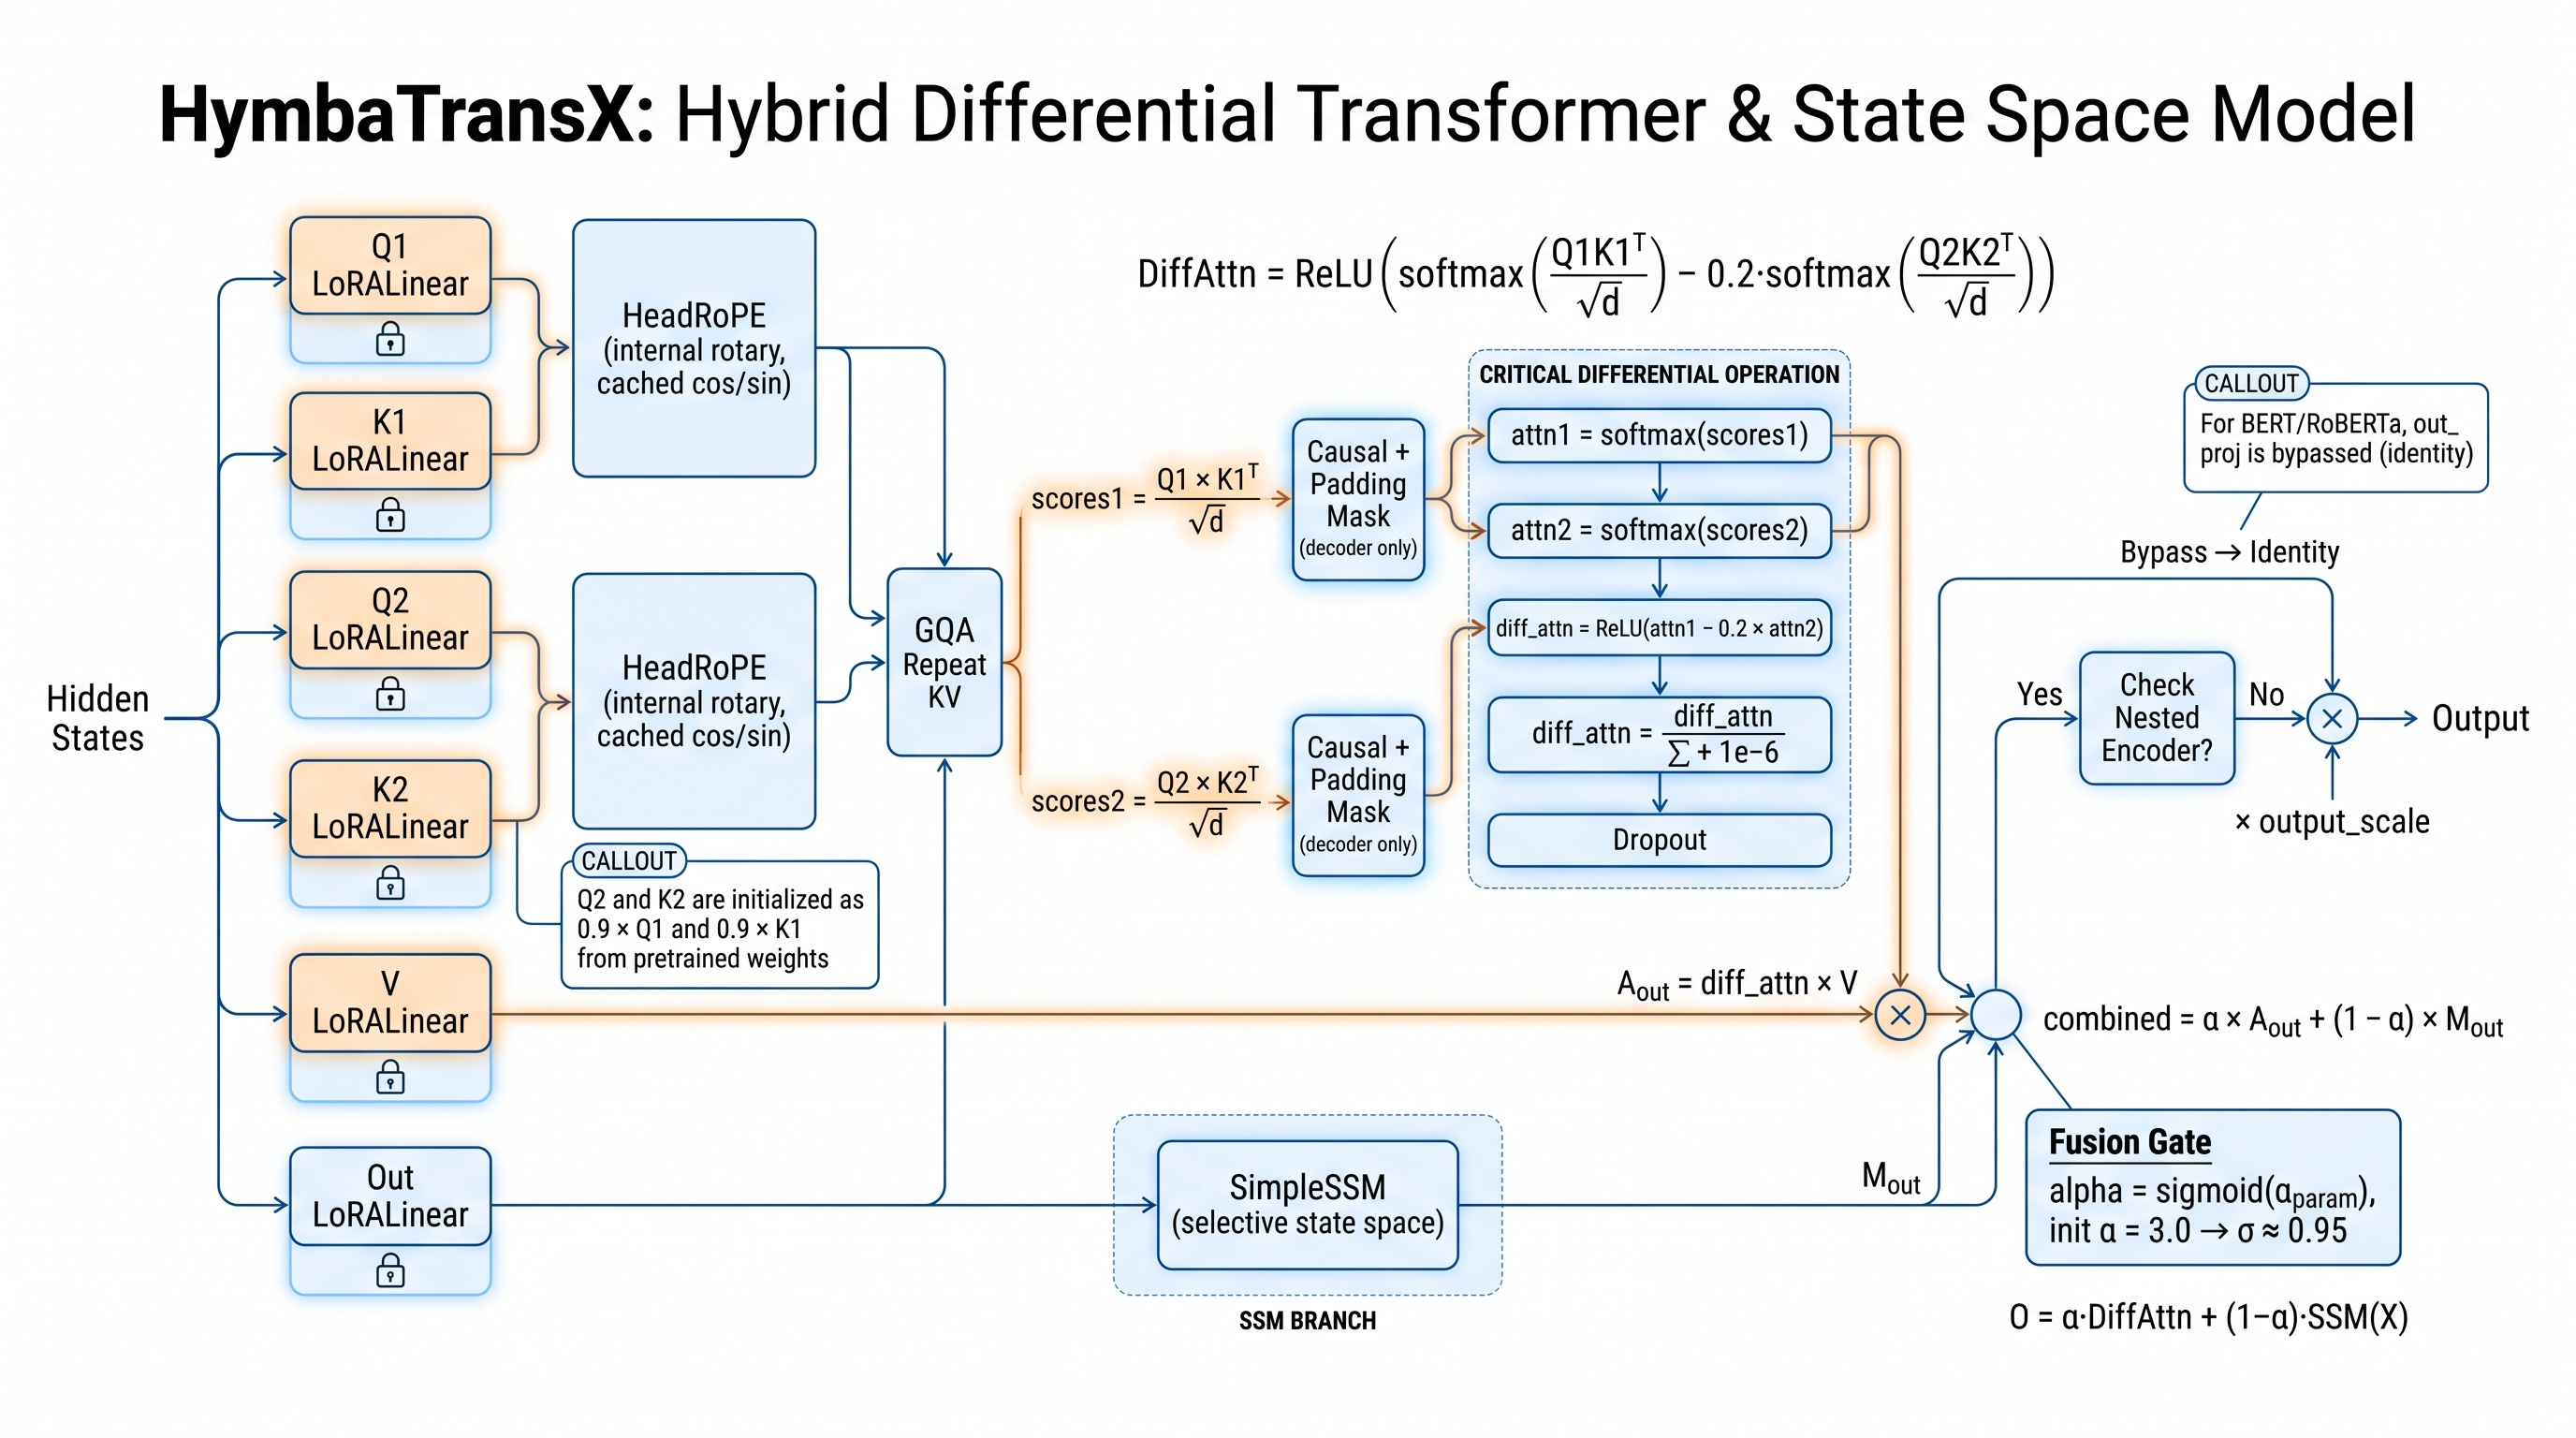
\includegraphics[width=0.92\textwidth]{img/arch_hymba_transx.jpeg}
\caption{دیاگرام ساختار معماری و جریان تانسوری ماژول \lr{(hymba\_transx)}}
\label{fig:arch_hymba_transx}
\end{figure}

\begin{figure}[H]
\centering
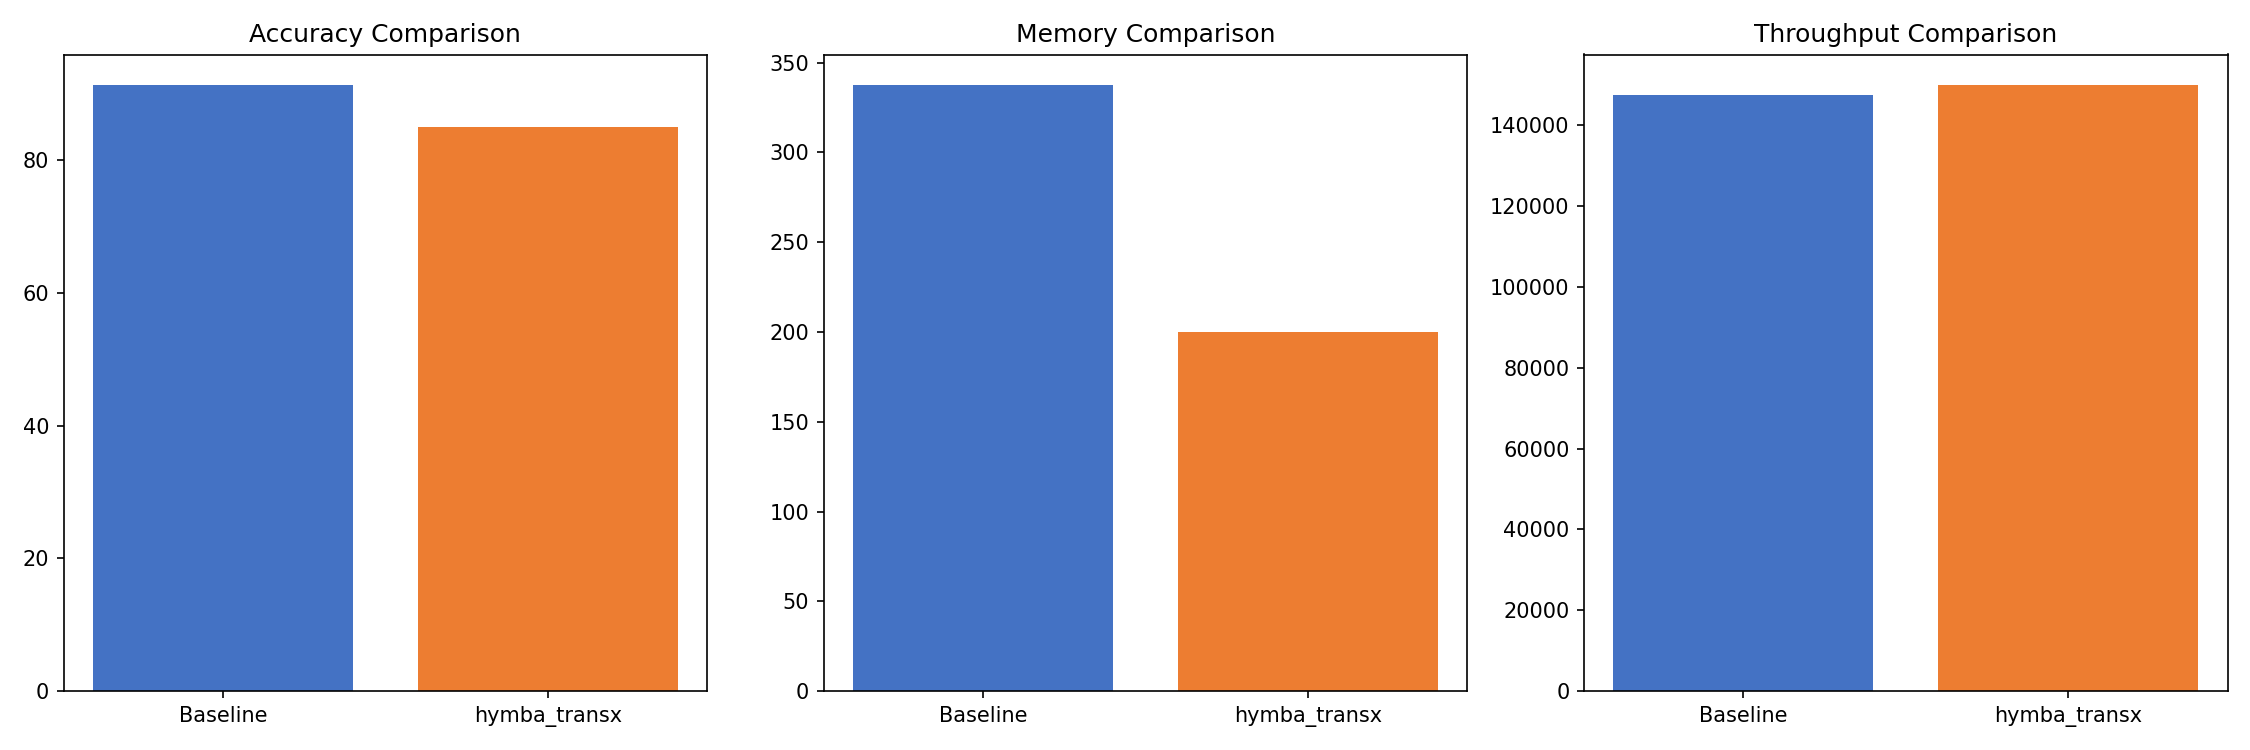
\includegraphics[width=0.92\textwidth]{img/comparison/hymba_transx_comparison.png}
\caption{نمودار ارزیابی مقایسه‌ای سه‌شاخصی مکانیزم در برابر خط مبنا \lr{(hymba\_transx)}}
\label{fig:comp_hymba_transx}
\end{figure}


\paragraph{تحلیل طیفی و نامساوی‌های پایداری خطا}
برای بررسی میزان دقت تقریب ماتریس وزن یا نگاشت توجه در ماژول \lr{hymba\_transx}، تفاضل ماتریس فاکتورگیری‌شده از نگاشت متراکم اصلی بر اساس نامساوی هافدینگ-فون‌نیومان ارزیابی می‌گردد. فرض کنید $\mathbf{W} \in \mathbb{R}^{d_{\text{in}} \times d_{\text{out}}}$ ماتریس وزن هدف باشد که توسط تقریب کم‌مرتبه یا پراکنده با رتبه موثر $r$ جایگزین شده است. کران بالای خطای بازسازی بر مبنای نرم فروبنیوس به صورت زیر تصریح می‌شود:
\begin{equation}
\label{eq:spectral_bound_hymba_transx}
\| \mathbf{W} - \mathbf{W}_{r} \|_F = \sqrt{\sum_{i=r+1}^{\min(d_{\text{in}}, d_{\text{out}})} \sigma_i^2(\mathbf{W})} \le \epsilon \| \mathbf{W} \|_F
\end{equation}
که در آن $\sigma_i(\mathbf{W})$ بیانگر $i$-امین مقدار منفرد مرتب‌شده ماتریس به صورت نزولی است. نسبت حفظ انرژی طیفی $\eta_r = \frac{\sum_{i=1}^r \sigma_i^2}{\sum_{i=1}^{d} \sigma_i^2}$ تضمین می‌کند که با انتخاب آستانه $\tau \ge 0.90$، بیش از نود درصد از پراکندگی واریانس داده‌ها حفظ شده و افت سیگنال در انتشار گرادیان رو به عقب به حداقل ممکن کاهش می‌یابد.

\paragraph{تحلیل مجانبی و پیچیدگی اشتراک حافظه سخت‌افزاری}
از منظر پیچیدگی محاسباتی و انتقال داده‌ها در سلسومراتب حافظه (حافظه سراسری \lr{HBM} به حافظه محلی \lr{SRAM})، عملیات ضرب ماتریسی در این مکانیزم نیازمند تخصیص بافر موقت با ابعاد فاکتورگیری‌شده است. برای پردازش دنباله‌ای به طول $N$ با بعد مخفی $D$، بار محاسباتی هسته از فرم درجه دو به رابطه زیر تقلیل می‌یابد:
\begin{equation}
\label{eq:complexity_hymba_transx}
\mathcal{C}_{\text{hymba\_transx}} = \mathcal{O}\left( B \cdot N \cdot D \cdot r + B \cdot H \cdot N \cdot d_k \right) \ll \mathcal{O}\left( B \cdot H \cdot N^2 \cdot d_k \right)
\end{equation}
این بهبود مرتبه پیچیدگی، با کاهش چشمگیر حجم تبادل تانسورها در گذرگاه‌های ارتباطی کارت گرافیک، مانع از اشباع پهنای باند حافظه (پدیده \lr{Memory-Bound}) در فرآیند استنتاج طولانی‌مدت می‌گردد.